\documentclass[../report.tex]{subfiles}

\begin{document}

\begin{figure}
\centering
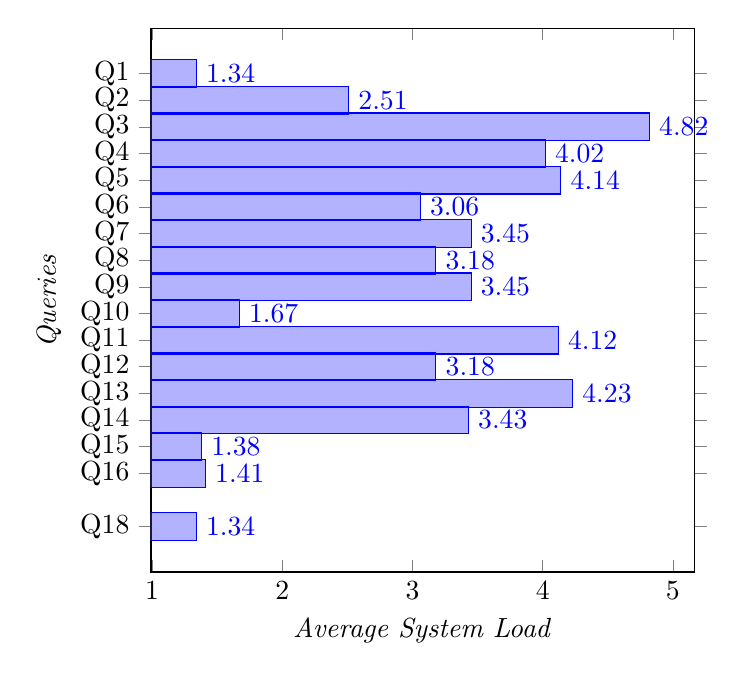
\begin{tikzpicture}[baseline]
    \begin{axis}[
            xbar,
            ytick=data,
            width=0.7\textwidth,
            height=0.7\textwidth,
            symbolic y coords={Q1,Q2,Q3,Q4,Q5,Q6,Q7,Q8,Q9,Q10,Q11,Q12,Q13,Q14,Q15,Q16,Q17,Q18,Q19,Q20,Q21,Q22},
            ylabel=\emph{Queries},
            xlabel=\emph{Average System Load},
            % xmode=log,
            y dir=reverse,
            nodes near coords,
            nodes near coords align={horizontal},
        ]
        \addplot coordinates {
            (1.34,Q1) (2.51,Q2) (4.82,Q3) (4.02,Q4) (4.14,Q5) (3.06,Q6) (3.45,Q7) (3.18,Q8) (3.45,Q9) (1.67,Q10) (4.12,Q11) (3.18,Q12) (4.23,Q13) (3.43,Q14) (1.38,Q15) (1.41,Q16) (1.34,Q18)
        };
    \end{axis}
\end{tikzpicture}
\label{fig:pg_load}
\caption{System load during running}
\end{figure}

\end{document}
